Model uczenia maszynowego jaki został wykorzystany w testach to sieć neuronowa.

Do testów stworzone zostało kilka modeli sieci neuronowych,
wytrenowanych na rysunkach grafów stworzonych za pomocą skryptów R.
Implementacja została wykonana biblioteką TensorFlow oraz Keras w języku Python.
Modele są w stanie rozpoznawać rysunki grafów i przypisywać im odpowiednie klasy.
Celem było również przetestowanie modeli na rzeczywistych zdjęciach,
zawierających wzorce przypominające grafy, bądź rysunkach grafów narysowanych ręcznie.

Stworzone zostały 3 modele:
- wytrenowany na danych ze stałą liczbą wierchołków
- wytrenowany na danych ze stałą liczbą wierchołków oraz walidacją krzyżową
- wytrenowany na danych ze zmienną liczbą wierzchołków

\subsection{Generacja danych}
Dane wygenerowane zostały przy pomocy skryptu stworoznego w języku R oraz biblioteki igraph.
Skrypt został zaprojektowany funkcyjnie, by osiągnąć możliwie największą automatyzację testów.
Rysunki grafów tworzone są o wielkości 800x600 pikseli, na białym tle, z wierzchołkami w kolorze pomarańczowym,
bez jakichkolwiek oznaczeń wierzchołków oraz zapisywane są w odpowiednich katalogach, odpowiadających klasie grafu.
Przygotowane zostały funkcje tworzące ścieżki, grafy cykliczne, grafy pełne, grary spójne, grafy dwudzielne oraz puste.
W każdej z funkcji możliwy jest wybór liczby generowanych grafów, liczba wierzchołków grafu
oraz współczynnik odpowiadający za zakrzywienie krawędzi na rysunkach.

W testach wykorzystane zostały wszystkie typy grafów.
Każdy z nich, czyli dana liczba wierchołków i typ grafu, wygenerowany został w liczbie 500 sztuk
oraz ze stałą krzywizną krawędzi, wynoszącą 0,3.

\subsection{Dane zewnętrzne}
Obrazy testowe, które nazwane są tutaj danymi zewnętrznymi, są rysunkami grafów pochodzącymi spoza przygotowanego testu.
Dzielą się na obrazy pobrane z internetu, obrazy wygenerowane przez skrypt w R, ale nie używane w treningu
oraz rysunki odręczne grafów.

\subsection{Opis skryptu}

\subsubsection{Przygotowanie}
Skrypt rozpoczyna się od przygotowania środowiska do trenowania modelu.
Najpierw ustawia ścieżki do katalogów z wygenerowanymi grafami oraz do katalogów na dane treningowe i walidacyjne.
Następnie sprawdza, czy te katalogi istnieją, a jeśli nie, tworzy je.
Dalej, definiuje parametry dotyczące wielkości obrazów oraz wielkości partii danych, które będą używane podczas treningu.
Dla każdej wartości liczby wierzchołków ustawia ścieżkę do katalogu z wygenerowanymi grafami,
pobiera listę podkatalogów oraz obrazów w każdym z nich,
a następnie dzieli obrazy na zestawy treningowe i walidacyjne w stosunku 80:20.
Tworzy odpowiednie katalogi dla tych zestawów, jeśli jeszcze nie istnieją,
i kopiuje obrazy do właściwych lokalizacji, segregując je na treningowe i walidacyjne.

\subsubsection{Model}
Na początku dane zostały przygotowane ze zbioru obrazów, znajdującego się w katalogu lokalnym.
Dokonany został podział na zbiory treningowe i walidacyjne.
Dla każdego przejścia walidacji krzyżowej, dane zostały podzielone inaczej.
Po wczytaniu danych, zostały przeskalowane i przeskztałcone do odcieni szarości.

Model sieci neuronowej został zdefiniowany jako sekwencyjny stos warstw.
Pierwsza warstwa to warstwa Rescaling, która normalizuje wartości pikseli do zakresu [0, 1].
Następne trzy warstwy to Conv2D z wybraną liczbą filtrów, z których każda jest poprzedzona warstwą MaxPooling2D.
Warstwy konwolucyjne używają różnych funkcji akytwacji, np. ReLU.
Po warstwach konwolucyjnych znajduje się warstwa Flatten, która przekształca mapy cech 2D w wektor 1D.
Następnie dodana jest w pełni połączona (Dense) warstwa z wybraną liczbą jednostek
i wybraną funkcją aktywacji, wraz z warstwą dropout.
Zastosowana jest tam również regularyzacja L2 (zmniejszanie wag) z ustaloną siłą regularyzacji wynoszącą.
Warstwa wyjściowa zawiera tyle jednostek, ile występuje klas.
Zależnie od danego testu, może być to różna liczba.

Dla standaryzacji danego testu ustalono K-Fold z liczbą podziałów równą 5.
Dla wszystkich warstw wybrana została funkcja aktywacji ReLU.
Liczba epok wyniosła 75.
W przypadku warstw konwolucyjnych, wybrano 32 filtry, a dla warstwy w pełni połączonej zastosowano 128 jednostek.
Regularyzacja została zastosowana z siłą 0,01, a współczynnik dropout - 0,2.

\subsubsection{Wyniki}
Po wytrenowaniu modelu, skrypt wizualizuje dokładność i stratę modelu.
Najpierw wyświetla w konsoli wartości dokładności dla obu zbiorów z historii treningu.
Dalej tworzy wykresy, gdzie na pierwszym z nich pokazuje dokładność na zbiorze treningowym i walidacyjnym,
a na drugim wykresie prezentuje stratę modelu dla obu zbiorów.

\subsubsection{Testy na danych zewnętrznych}
Po wyświetleniu dokładnosci modelu skrypt przeszukuje katalog z danymi i jego podkatalogi, by przygotować obrazy zewnętrzne.
Następnie ustawia ścieżkę do katalogu z obrazami testowymi i pobiera ich listę.
Dla każdego obrazu w tej liście wczytuje go, przeskalowuje do odpowiedniego rozmiaru i konwertuje do skali szarości
Następnie model przewiduje klasę obrazu, a wynik jest wyświetlany w konsoli.

\subsection{Testy modeli}
\subsubsection{Model podstawowy}

\begin{figure}[ht]
	\centering
	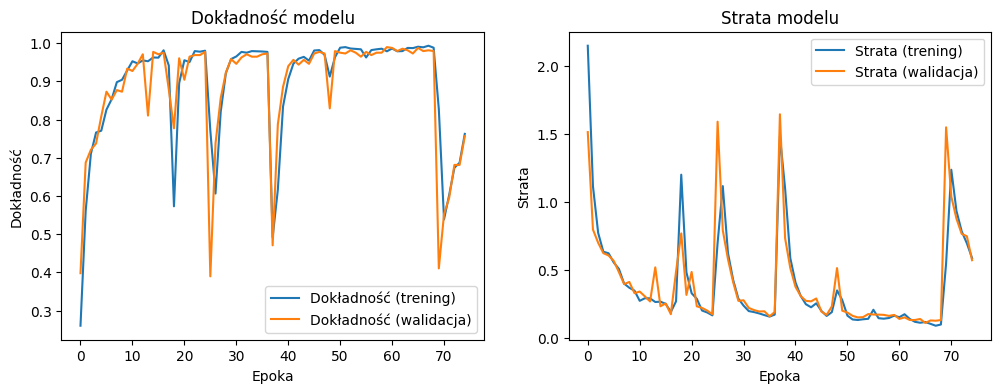
\includegraphics[height=5.5cm]{partials/images/tests/v2_epoch75.png}
	\caption{Wyniki testów dla modelu podstawowego}
\label{Fig:GraphUndirected}
\end{figure}
\FloatBarrier

\begin{figure}[ht]
	\centering
	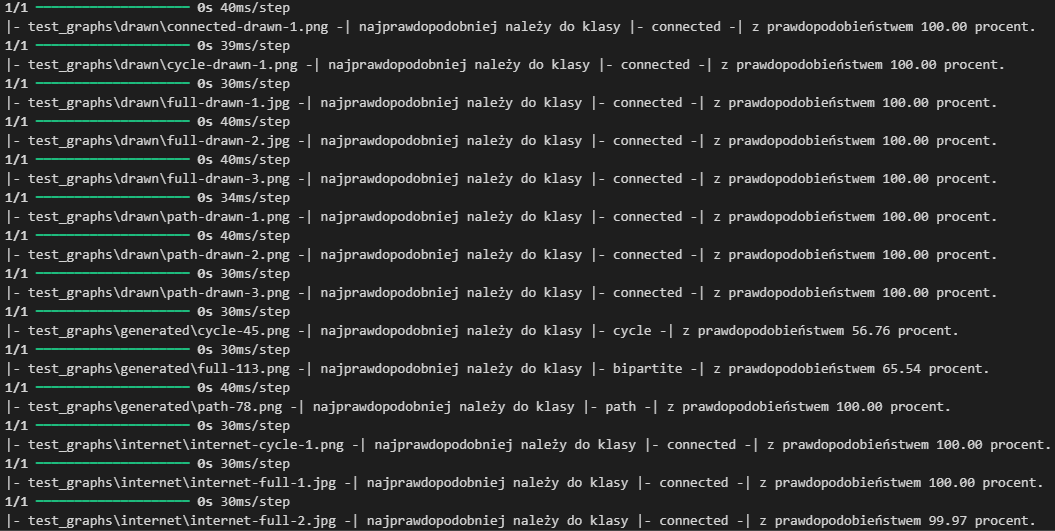
\includegraphics[height=7cm]{partials/images/tests/v2_epoch75_img_tests.png}
	\caption{Klasyfikacja obrazów zewnętrznych dla modelu ze zmienną liczbą wierzchołków}
\label{Fig:GraphUndirected}
\end{figure}
\FloatBarrier

\subsubsection{Model z walidacją krzyżową}

W przypadku standardowego modelu z walidacją krzyżową model bardzo szybko uległ przeuczeniu.
Już po szóstej iteracji dokładność na zbiorze walidaycjnym wyniosła 100\%, co nie jest realistycznie możliwe.
Została podjęta próba ograniczenia overfittingu poprzez zwiększenie zbioru danych, zmiany liczby epok w modelu
oraz manipulacji współczynnikami dropout i regularyzacji.
W każdym przypadku model zwracał niezadowalające wyniki wynoszące 100\% po jednej z początkowych iteracji.

\begin{figure}[ht]
	\centering
	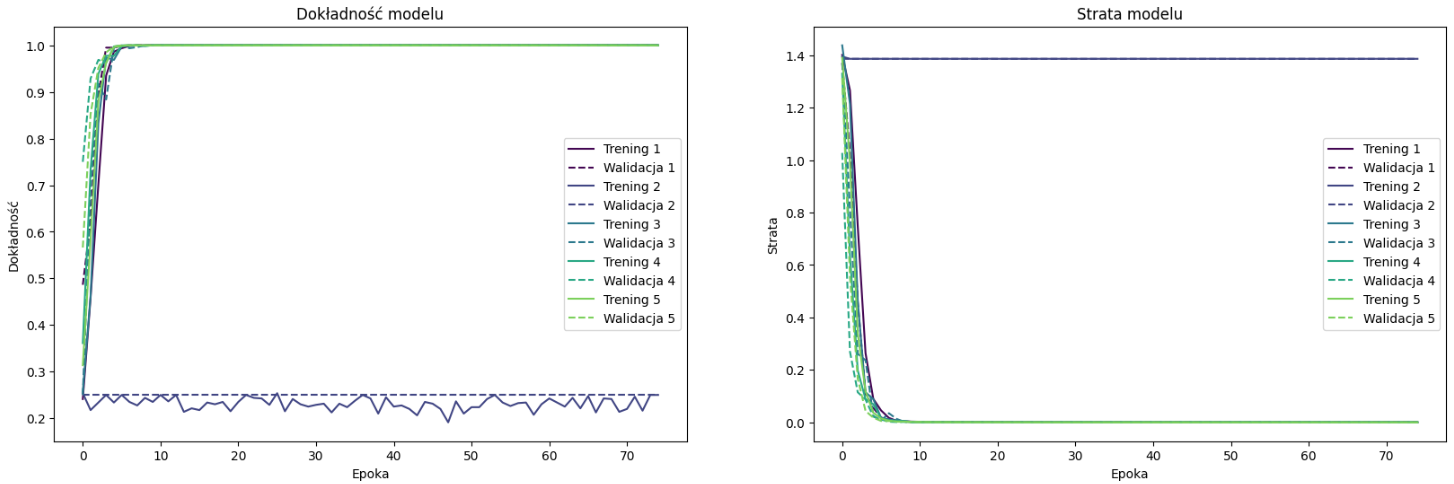
\includegraphics[height=5.5cm]{partials/images/tests/v2_crossvalid.png}
	\caption{Wyniki testów dla modelu z walidacją krzyżową}
\label{Fig:GraphUndirected}
\end{figure}
\FloatBarrier

Z powodu przeuczenia model nie radził sobie z zewnętrznymi obrazkami testowymi.
Większość grafów określił jako grafy pełne, co nie jest zgodne ze stanem rzeczywistym.

\begin{figure}[ht]
	\centering
	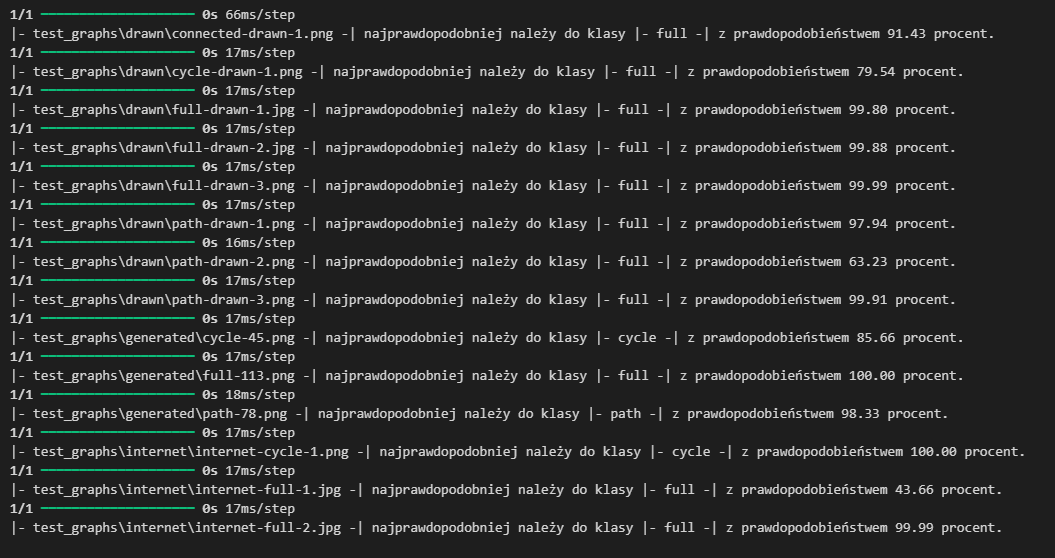
\includegraphics[height=7cm]{partials/images/tests/v2_crossvalid_img_tests.png}
	\caption{Klasyfikacja obrazów zewnętrznych dla modelu z walidacją krzyżową}
\label{Fig:GraphUndirected}
\end{figure}
\FloatBarrier

\subsubsection{Model ze zmienną liczbą wierzchołków}
Najlepsze wyniki pod względem rozpoznawania zewnętrznych obrazków testowych
oraz realistycznej dokładności na zbiorze walidacyjnym,
zostały uzyskane przy użyciu modelu sieci neuronowej uczonej na rysunkach grafów z różną liczbą wierzchołków.
Było to odpowiednio 4, 5, 6 oraz 7 wierzchołków.

\begin{figure}[ht]
	\centering
	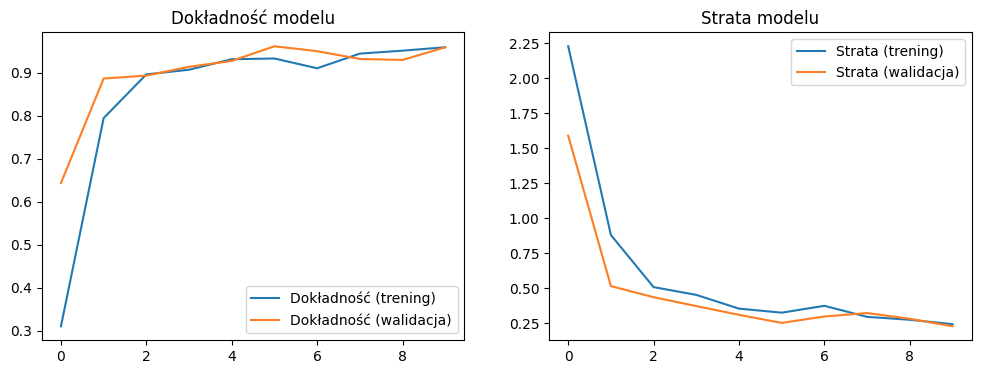
\includegraphics[height=5.5cm]{partials/images/tests/v2_multiple_edges.png}
	\caption{Wyniki testów dla modelu ze zmienną liczbą wierzchołków}
\label{Fig:GraphUndirected}
\end{figure}
\FloatBarrier

Model nie poradził sobie zbyt dobrze z obrazami zewnętrznymi, lecz znacznie lepiej niż model z walidacją krzyżową.
Poprawnie wskazanych klas grafów było 5 z 14 wszystkich rysunków.
Mimo, że model jest w stanie poprawnie określić niektóre typy grafów poprawnie,
wciąż jest to dokładność niższa niż 50\%.

\begin{figure}[ht]
	\centering
	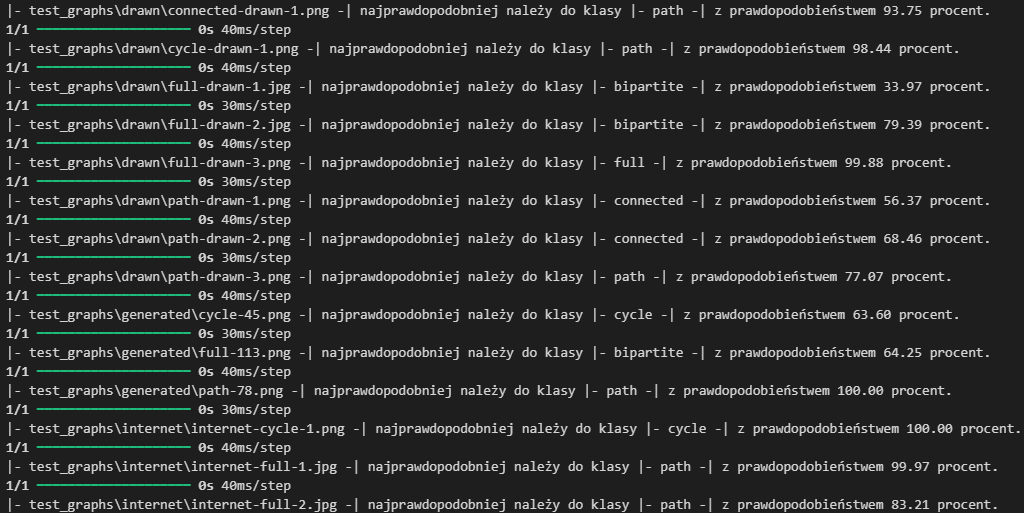
\includegraphics[height=7cm]{partials/images/tests/v2_multiple_edges_img_tests.png}
	\caption{Klasyfikacja obrazów zewnętrznych dla modelu z walidacją krzyżową}
\label{Fig:GraphUndirected}
\end{figure}
\FloatBarrier

\subsubsection{Model ze zmienną liczbą wierzchołków i walidacją krzyżową}

\begin{figure}[ht]
	\centering
	% \includegraphics[height=5.5cm]{partials/images/tests/v2_multiple_edges_crossvalid.png}
	\caption{Wyniki testów dla modelu ze zmienną liczbą wierzchołków i walidacją krzyżową}
\label{Fig:GraphUndirected}
\end{figure}
\FloatBarrier

\begin{figure}[ht]
	\centering
	% \includegraphics[height=5.5cm]{partials/images/tests/v2_multiple_edges_crossvalid_img_tests.png}
	\caption{Klasyfikacja obrazów zewnętrznych dla modelu ze zmienną liczbą wierzchołków i walidacją krzyżową}
\label{Fig:GraphUndirected}
\end{figure}
\FloatBarrier

\subsection{Wnioski}
W przypadku uczenia modeli z wykorzystaniem grafów pełnych, najczęściej dominowały one cały zbiór danych,
przez co modele w kolejnych testach klasyfikowały większość testowych grafów rysowanych odręcznie jako właśnie grafy pełne.

Testy z wykorzystaniem stałej liczby wierzchołków grafów okazały się mniej owocne niż testy z rysunkami grafów
o zmiennej liczbie wierchołków.

Wystąpiła tendencja do niepoprawnego określania innych grafów, grafami dwudzielnymi, jeśli takie znajdowały się
w zbiorze danych uczących.